\section{Introduction}
\label{sec:svbrdf:intro}

Despite a few decades of effort in computer graphics and vision, capturing spatially-varying reflectance of real-world materials remains a challenging and actively researched task.
Measurement methods have traditionally used custom hardware systems to densely sample illumination and viewing directions \cite{marschner1999image,matusik2003data}, followed by post-processing such as fitting parametric BRDF models \cite{ngan2005experimental}. However, such approaches are restricted to laboratory conditions.

Recent work has explored methods for casual capture of spatially-varying BRDFs (SVBRDFs) using commodity hardware and in less constrained environments \cite{Francken2009,Ren2011,Aittala2013,Aittala2015,Hui2017}.
These methods usually follow an \emph{inverse-rendering} approach: they define a forward rendering model and optimize reflectance parameters so that the simulated appearance matches physical measurements under certain image metrics.
With a small number of measured images, this approach is fundamentally under-constrained: there usually exist many material estimates capable of producing renderings that match the measurements, but many of these estimates can be unrealistic and may not generalize to novel illumination and viewing conditions.
The solution to this problem has been to \emph{regularize} the optimization using pre-determined \emph{material priors} such as linear low-dimensional BRDF models \cite{Ren2011,Hui2017} or stationary stochastic textures \cite{Aittala2015,Aittala2016}.
However, such hand-crafted priors do not generalize to a wide range of real-world materials.

More recently, learning-based approaches have demonstrated remarkable results for reconstructing SVBRDFs from one \cite{Deschaintre2018,Li2018} or more images \cite{Deschaintre2019}.
While these methods use rendering-based losses (similar to the inverse rendering approaches) during training, at test time they predict SVBRDFs from images using a single feed-forward pass through a deep network.
As a result, the reconstructed material parameters may not accurately reproduce the measured appearance.
In contrast, Gao et al. \cite{Gao2019} propose using an optimization-based approach in conjunction with a learned material prior.
Specifically, they train a fully-convolutional auto-encoder on a large material dataset and optimize in the latent space of this auto-encoder. This ensures that the reconstructed SVBRDF parameters both reproduce the measurements and are plausible real-world materials.
However, while this learned material prior is a significant improvement over hand-crafted priors, it still produces a relatively localized and highly flexible latent space that requires a good initialization (for example, from single image methods \cite{Deschaintre2018,Li2018}) and even then can fail to produce good results.

In this paper, we propose a different material prior that builds on the remarkable progress in image synthesis using deep Generative Adversarial Networks (GANs) \cite{Goodfellow2014,Karras2018,StyleGAN}.
We train \emph{MaterialGAN}---a StyleGAN2-based deep convolutional neural network \cite{StyleGAN2}---to generate plausible materials from a large-scale, spatially-varying material dataset \cite{Deschaintre2018}.
MaterialGAN learns \emph{global} correlations in material parameters, both spatially (thus encoding texture patterns) as well as across parameters (for example, relationships between diffuse and specular parameters).
As illustrated in Figure~\ref{fig:svbrdf:matgan}, sampling from the MaterialGAN latent space produces plausible, realistic materials with complex variations and diverse appearance.

\begin{figure}[h]
	\centering
	\setlength{\resLen}{0.85in}
	\addtolength{\tabcolsep}{-4pt}
	\begin{tabular}{ccccccc}
		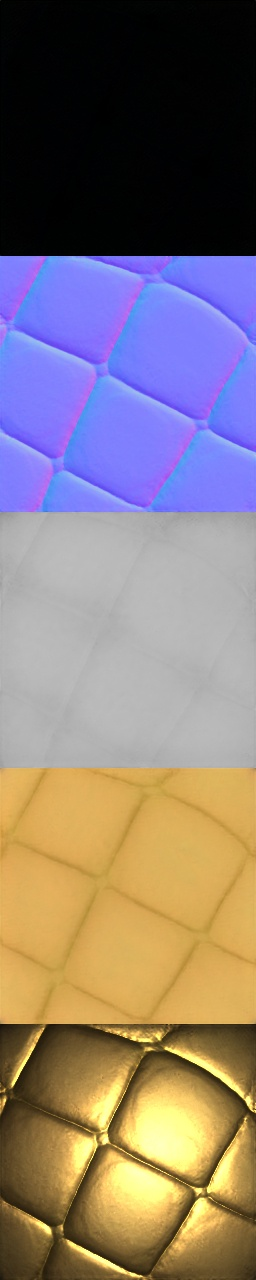
\includegraphics[width=\resLen]{svbrdf/others/matgan/04.jpg} &
		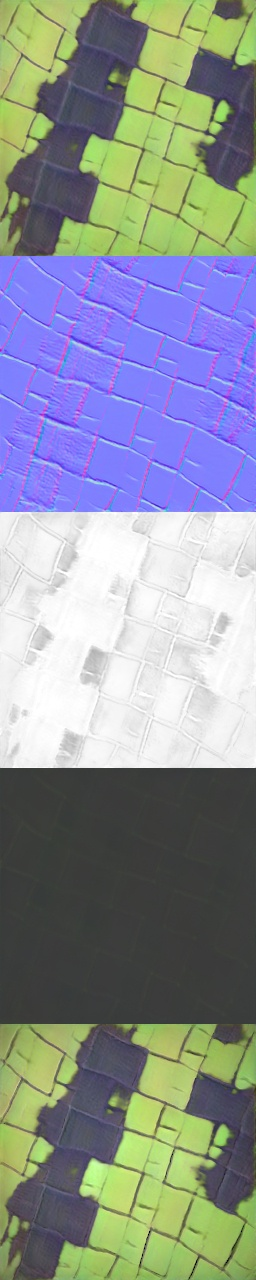
\includegraphics[width=\resLen]{svbrdf/others/matgan/05.jpg} &
		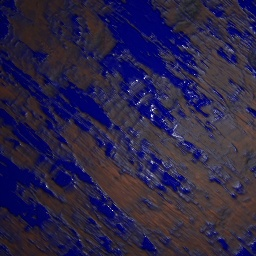
\includegraphics[width=\resLen]{svbrdf/others/matgan/08.jpg} &
		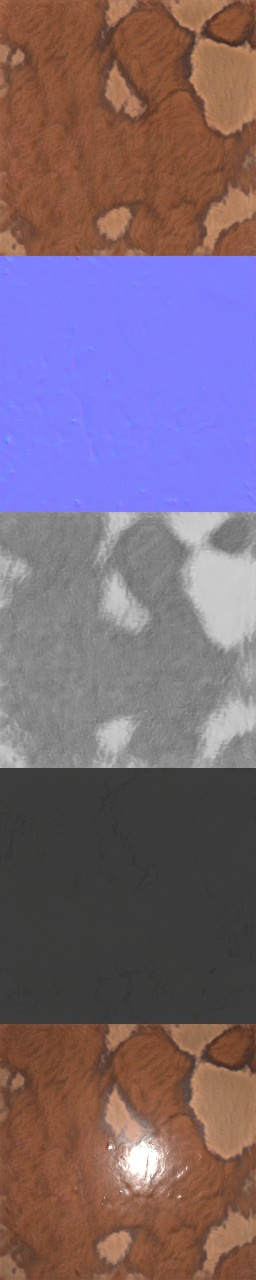
\includegraphics[width=\resLen]{svbrdf/others/matgan/10.jpg} &
		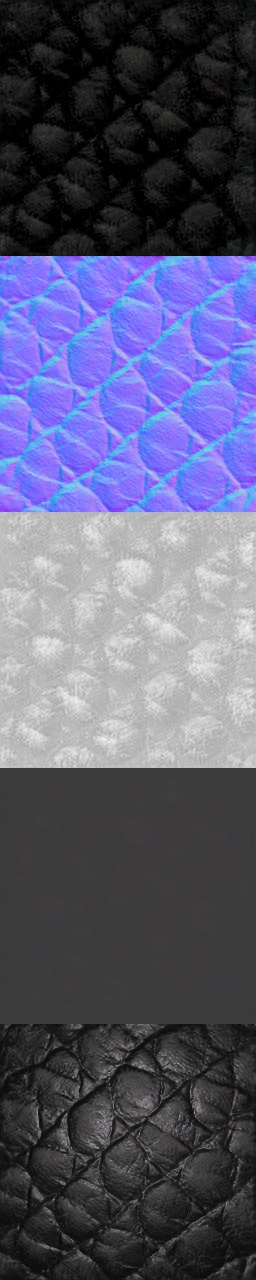
\includegraphics[width=\resLen]{svbrdf/others/matgan/11.jpg} &
		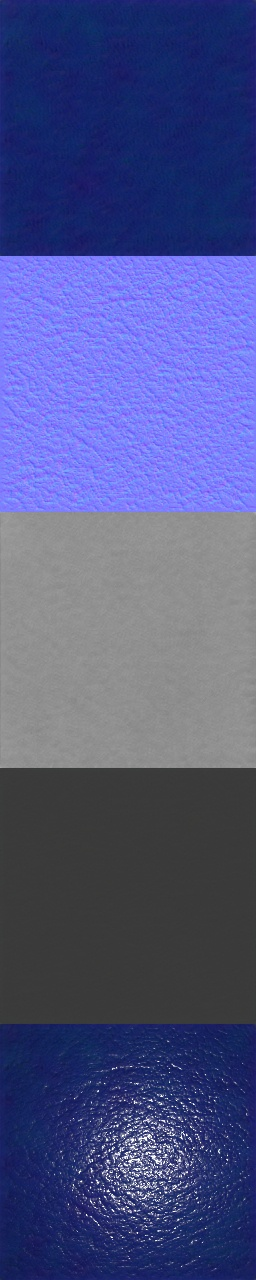
\includegraphics[width=\resLen]{svbrdf/others/matgan/12.jpg} &
		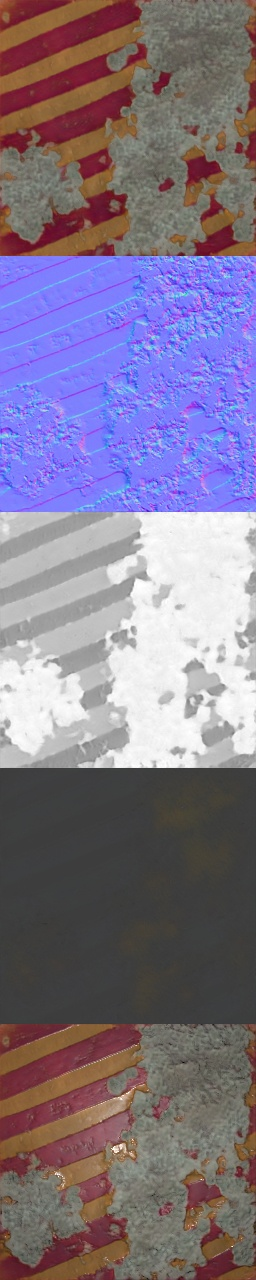
\includegraphics[width=\resLen]{svbrdf/others/matgan/19.jpg}
	\end{tabular}
	\caption[Materials generated by MaterialGAN]{\label{fig:svbrdf:matgan}
		\textbf{Seven materials generated by randomly sampling MaterialGAN.} Top to bottom: diffuse albedo, normal, roughness, specular albedo and renderings under flash illumination. As can be seen, the material maps are high-quality with meaningful correlations both spatially and across materials parameters, and visually look like plausible real-world materials.
	}
\end{figure}

While GANs have traditionally been used to synthesize images, we demonstrate a very different application, using MaterialGAN as a powerful prior in an inverse rendering-based material capture framework.
We append a rendering layer to MaterialGAN, setting up a differentiable pipeline from the learned latent space, through generating material maps, to rendering images under specified views and lighting.
This allows us to optimize the MaterialGAN latent vector(s) to minimize the error between the rendered and measured images and reconstruct the corresponding material maps.
Doing so ensures that the reconstructed SVBRDFs lie on the ``manifold of realistic materials'', while at the same time accurately reproducing the captured images.

We demonstrate that our GAN-based optimization framework produces high-quality SVBRDF reconstructions from a small number (3-7) images captured under flash illumination using hand-held mobile phones, and improves upon previous state-of-the-art methods \cite{Gao2019,Deschaintre2019}.
In particular, it produces cleaner, more realistic material maps that better reproduce the appearance of the captured material under both input \emph{and novel} lighting.
Moreover, as illustrated in Figure \ref{fig:svbrdf:real}, MaterialGAN adapts to a wide range of SVBRDF samples ranging from diffuse to specular materials and near-stochastic textures to structured patterns with multiple distinct, complex materials.

Furthermore, our GAN-based latent space offers the ability to edit the latent vector in semantically meaningful ways (via operations like interpolation in the latent space) and generate realistic materials that go beyond the captured images.
This is not possible with current material capture methods that do not afford any control over their per-pixel BRDF estimates.

